\section{Discussão}
\label{sec:discussao}

\subsection{Ótimos locais e ótimo global}

Na instância pequena, a descida gulosa encontra poucos ótimos locais distintos (Tabela~\ref{tab:otimos}).
Nas 30 execuções, a \textit{best} e a \textit{first improvement} terminaram cerca de 1\,500 e 4\,100 descidas, mas em só 19 permutações diferentes cada uma, e de 11\% a 15,5\% delas terminam no ótimo global.
Com dezenas de reinícios por execução, achar $h^*$ em todas era quase certo.
A paisagem tem poucas bacias, uma delas a do ótimo, o que favorece quem reinicia muitas vezes.
O SA também acha $h^*$ em todas as execuções, por outro caminho: atravessa as barreiras entre bacias aceitando pioras.
O AG acha o ótimo em 12 das 30, porque a população converge antes que algum indivíduo chegue ao fundo da bacia (Seção~\ref{sec:exploracao}).
As 491 paradas distintas da variante \textit{random} não contradizem o quadro: ela para depois de $K$ sorteios sem melhoria, e muitas dessas paradas não são ótimos locais.

\begin{table}[tbp]
  \centering
  \caption{Instância pequena: ótimos locais da descida gulosa (médias por execução, total distinto nas 30 execuções, fração das descidas que terminam em $h^*$) e execuções que atingiram $h^* = 1\,875$.}
  \label{tab:otimos}
  \tabela{otimos_locais}
\end{table}

\subsection{Exploração e intensificação}
\label{sec:exploracao}

Na \textbf{descida gulosa}, o reinício explora e a descida intensifica, e o equilíbrio depende de quantas descidas cabem no orçamento (Tabela~\ref{tab:gd-variantes}).
A \textit{first improvement} completa 10,3 descidas por execução na média e 1,4 na grande.
A \textit{best improvement} paga a vizinhança inteira a cada passo (22\,201 avaliações em $n = 150$) e dá 13 passos de melhoria em 300\,000 avaliações, quando uma permutação aleatória precisa de mais de mil para chegar a um ótimo local.
Na grande, ela termina com mediana de 818\,369,5, pior que o guloso construtivo (398\,095); na média, já perde para as outras variantes ($p = 7{,}0\times10^{-9}$).
A \textit{first} e a \textit{random} dão mais de mil passos por execução e empatam entre si: com orçamento fixo, escolher o melhor sucessor não compensa o preço de examinar todos.

\begin{table}[tbp]
  \centering
  \caption{Variantes da descida gulosa: passos de melhoria, descidas iniciadas e descidas que terminaram em ótimo local (médias por execução), mediana do melhor $h$ e teste contra a variante \textit{random}.}
  \label{tab:gd-variantes}
  \tabela{gd_variantes}
\end{table}

No \textbf{SA}, a temperatura faz a troca.
A aceitação de pioras (Figura~\ref{fig:sa}) começa em 0,87, cai para 0,19 na metade do orçamento e termina entre 0,002 e 0,006, o perfil de passeio aleatório que vira descida que a calibração buscava.
As três curvas praticamente coincidem, embora $T_0$ vá de 5\,481 a 63\,416: calibrar pelo perfil de aceitação neutralizou a diferença de escala de $\Delta$.
O preço está na Figura~\ref{fig:convergencia}: metade do orçamento passa com $h$ muito acima do da descida gulosa, e a última melhoria acontece, na mediana, depois de 98\% do orçamento na média e na grande.
O SA termina ainda melhorando, e com $2B$ foi o que mais ganhou na grande (de 80\,832,5 para 76\,488,5; Tabela~\ref{tab:robustez}).
Na grande, portanto, o equilíbrio pende para a exploração; um $T_0$ menor anteciparia a intensificação, hipótese que não testamos.

\begin{figure}[tbp]
  \centering
  \begin{minipage}[b]{0.335\textwidth}
    \centering
    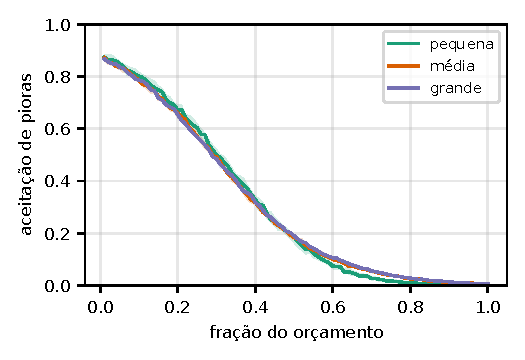
\includegraphics[width=\textwidth]{sa_aceitacao}
  \end{minipage}\hfill
  \begin{minipage}[b]{0.655\textwidth}
    \centering
    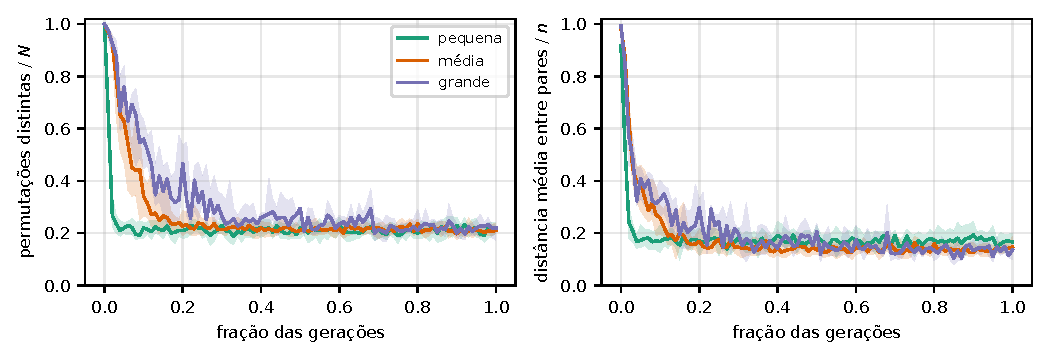
\includegraphics[width=\textwidth]{ag_diversidade}
  \end{minipage}
  \caption{À esquerda, SA: fração das pioras propostas que foram aceitas, por janela de $B/100$ passos. No centro e à direita, AG: permutações distintas como fração de $N$ e distância média entre 50 pares sorteados (posições diferentes) como fração de $n$. Mediana e intervalo interquartil das execuções.}
  \label{fig:sa}
\end{figure}

No \textbf{AG}, a população e o cruzamento exploram, e o torneio com elitismo intensifica.
Aqui o equilíbrio pendeu para a intensificação (Figura~\ref{fig:sa}).
Na pequena, a população de 50 cai para 11 permutações distintas antes de 5\% das gerações, e na média, para um terço em 10\%.
Nas três instâncias a diversidade estaciona perto de 20\%, praticamente os mutantes de cada geração ($P_m = 0{,}2$) em volta de cópias de um indivíduo, e a distância média entre pares cai para cerca de 15\% das posições.
A última melhoria do melhor indivíduo acontece, na mediana, com 3\% do orçamento na pequena e 48\% na média, e na média dar $2B$ ao AG não mudou o resultado de nenhuma das 30 execuções.
Só na grande, onde a população demora mais para convergir, ele ainda melhorava no fim.

\subsection{Efeito de escala}

A ordem não muda com o tamanho: descida gulosa e SA empatados, os dois à frente do AG nas três instâncias.
O que muda é a distância: o gap mediano do AG vai de 3,3\% a 18,7\% e 56\%, e o das buscas locais, de 0 a 4--6\% e 34\%.
Os testes sustentam a ordem só onde há diferença; o empate entre descida gulosa e SA é ausência de evidência de diferença, não evidência de igualdade, e com 10 execuções na grande o teste tem pouco poder.

O custo de examinar a vizinhança explica a maior parte do efeito.
Com $n = 12$, a vizinhança de inserção tem 121 sucessores e uma descida custa algumas centenas de avaliações; com $n = 150$, tem 22\,201 e uma descida custa da ordem de 200\,000.
O orçamento cresce 6 vezes da pequena para a grande, e o espaço de busca, de $10^{8}$ para $10^{262}$ permutações.
A \textit{best improvement}, cujo passo custa $O(n^2)$ avaliações, é a que mais sofre.
O SA não examina vizinhanças e teve a temperatura calibrada por instância, então a escala o atinge menos.
O AG faz poucas gerações para o tamanho do problema e converge longe dos ótimos locais.
Com $2B$ (Tabela~\ref{tab:robustez}) a ordem se manteve: as buscas locais melhoraram, e o AG estacionou na média e continuou atrás na grande.

\subsection{Quando o AG compensa?}

Em nenhuma instância: o AG perde para as duas buscas locais em todas.
O OX aposta que soluções boas compartilham subsequências úteis, como grupos de ativos próximos e com prazos parecidos visitados numa certa ordem, e que cruzar dois pais bons combina blocos bons.
Se a aposta falha, o cruzamento é só uma mutação grande.
Para separar as duas explicações, rodamos o AG em cinco versões, com o mesmo protocolo e as mesmas sementes:
OX (a principal);
PMX~\citep{goldberg1985alleles}, que preserva posições absolutas em vez da ordem relativa;
só mutação ($P_c = 0$);
\textit{headless chicken}~\citep{jones1995crossover}, em que o segundo pai é uma permutação aleatória, o que torna o cruzamento uma macromutação sem informação;
e um AG memético~\citep{moscato1989memetic}, em que cada filho, com probabilidade 0,1 (escolhida num piloto fora do protocolo), desce até um ótimo local por \textit{first improvement}, pagando uma avaliação por sucessor.

\begin{table}[tbp]
  \centering
  \caption{Experimento extra: variantes do AG. Testes de Mann--Whitney contra o AG-OX, com correção de Holm sobre as quatro comparações de cada instância.}
  \label{tab:extra}
  \tabela{extra}
\end{table}

Trocar o OX pelo PMX ou retirar o cruzamento não muda o AG de forma detectável ($p \ge 0{,}275$; Tabela~\ref{tab:extra} e Figura~\ref{fig:extra}, no apêndice), e na grande a versão só com mutação tem até a menor mediana.
O \textit{headless chicken} é muito pior que o OX na média e na grande ($p = 1{,}2\times10^{-10}$ e $7{,}3\times10^{-4}$), pior até que o guloso na grande.
O cruzamento, então, transmite informação do segundo pai, já que trocá-lo por ruído destrói o resultado, mas essa informação não acrescenta nada ao que mutação e seleção fazem sozinhas.
Nossa leitura é que um bloco bom num pai não é bom por si só: seu atraso depende do instante em que a equipe chega a ele, isto é, de tudo o que vem antes na rota.

Só a versão memética melhora o AG, nas três instâncias ($p$ com Holm de $3{,}3\times10^{-6}$, $5{,}6\times10^{-6}$ e $0{,}011$), e ela chega ao nível das buscas locais sem superá-las ($p$ com Holm de 1,000 contra as duas; Tabela~\ref{tab:extra-buscas}).
Com a busca local, o AG vira um gerador de pontos de partida para descidas, e o que ele acrescenta ao reinício aleatório não aparece nos dados.
Neste problema e com este orçamento, o AG não compensa; o que decide é a busca local, venha ela de reinícios, da temperatura ou dos filhos.
